\section*{Dati e risultati}

\subsection*{Corrente di attivazione}

Per stimare la corrente di attivazione ($I_0$) del nostro interruttore differenziale abbiamo montato il nostro circuito come mostrato in Figura \ref{fig:circuito}.
Quindi abbiamo variato il valore della resistenza ($R$) fino a che l'interruttore non avesse funzionato.
Naturalmente la precisione della stima del valore di resistenza è andata aumentando passo passo e, una volta trovato il valore minimo, abbiamo verificato più volte che tale risultato fosse corretto.
il valore che abbiamo ottenuto è stato di:

\begin{equation}
        R \,=\, 348 \pm 1 \,\si{\ohm}
\end{equation}

Quindi una volta trovato il valore di $R$ abbiamo sfruttato l'amperometro per effettuare una misura diretta dell'intensità di corrente del nostro circuito e abbiamo ottenuto il seguente valore per la corrente di attivazione (I\ped{exp}):

\begin{equation}
        I\ped{exp} \,=\, 22 \pm 1 \,\si{\milli\ampere}
\end{equation}

Per assicurarci che i valori ottenuti fossero plausubili abbiamo sfruttato la legge di Ohm per ricavare il valore ipotetico di corrente passante nel circuito assumendo come $R$ il valore precedentemente ottenuto. Il valore teorico di $I$ risulta essere il seguente:

\begin{equation}
        I\ped{teo} \,=\, 22 \pm 1 \,\si{\milli\ampere}
\end{equation}

Questo valore è stao ottenuto assumendo che il nostro generatore fosse affetto da un $5\%$ di errore. A primo acchito può sembrare alto, ma dal momento che nei calcoli non si è tenuto conto della resistenza interna degli strumenti e dell'interruttore differenziale forse tale incertezza non è del tutto ingiustificata.

\subsection*{Tempo di Intervento}

In questa seconada parte invece voglamo stimare il tempo di inervento ($\tau\ped{int}$) del nostro interruttore differenziale. Per farlo abbiamo impostato un valore di $R$ inferiore al minimo trovato in modo che l'interruttore scattasse non appena si fosse alimentato il circuito. Quindi grazie ai due sagnali in entrata all'oscilloscopio, uno dellla tensione in ingresso al circuito ($V\ped{in}$) e uno della tensione ai capi dell'interruttore ($V_0$) ci è possibile stimare il tempo di intervento dell'interruttore.

Infatti $V\ped{in}$ si presenta come un segnale sinusoidale fin dall'accensione del generatore, mentre $V_0$ risuta essere, giustamente, nullo fino a che non scatta l'interruttore. Da quel momento in poi il segnale di $V_0$ coinciderà con quello di $V\ped{in}$. Il tempo di intervento
è il tempo che intercorre tra il momento in cui la derivata della tensione supera una certa soglia (determinata dall'induttanza contenuta nell'interruttore) e il momento in cui viene effettivamente aperto il circuito. Pertanto non possiamo ottenere il tempo di intervento esatto, ma è possibile sovrastimarlo leggendo direttamente sull'oscilloscopio l'intervallo tra l'accensione del generatore e l'apertura del circuito.

Uno esempio significativo è riportato in Figura \ref{fig:graph}, e crediamo possa essere di aiuto nel capire quanto esposto in precedenza.

Abbiamo eseguito molte misure con resistenze differenti per randomizzare eventuali errori sistematici. Poiché i valori misurati fluttuano
selvaggiamente e sono completamente scorrelati con il valore della resistenza usata per misurarli, abbiamo preso la media aritmetica,
con relativo errore standard, come sovrastima del tempo di intervento:

\begin{equation*}
    \tau\ped{int} \,=\, 10 \pm 5  ~ \si{\milli\second}
\end{equation*}

\begin{SCfigure}
    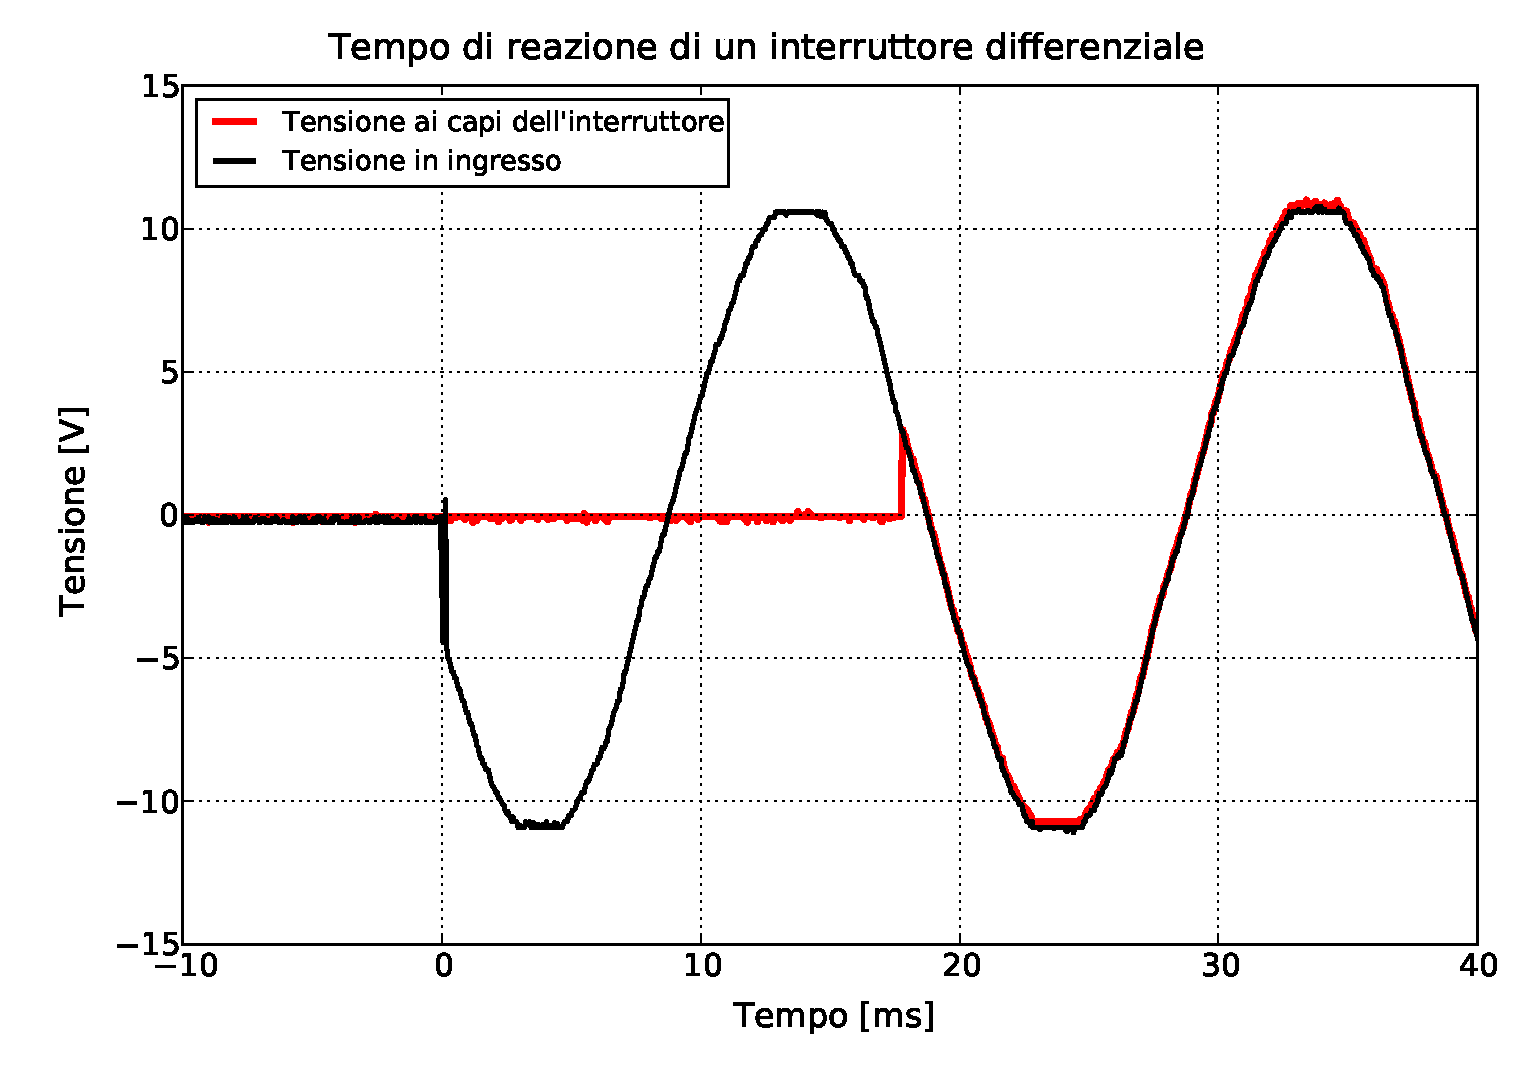
\includegraphics[scale=0.5]{tensione.pdf}
    \caption{Il grafico illustra le tensioni misurate nell'esperimento. Al tempo zero abbiamo acceso l'alimentatore.
    Fino all'apertura dell'interruttore, la tensione ai suoi capi è nulla, come evidenziato dalla linea rossa. Il tempo di intervento
    è il tempo che intercorre tra il momento in cui l'interruttore inizia a funzionare e il momento in cui viene effettivamente aperto
    il circuito. Purtroppo il tempo di inizio dell'intervento non è a noi accessibile, non conoscendo le specifiche
    interne dell'interruttore. Una sovrastima del tempo di intervento è data dal tempo trascorso tra l'accensione dell'alimentatore
    e l'apertura dell'interruttore, che in figura è circa 17 ms.}
    \label{fig:graph}
\end{SCfigure}
